\documentclass[a4paper, 11pt]{article}
\usepackage[utf8x]{inputenc}
\usepackage{comment} % enables the use of multi-line comments (\ifx \fi) 
\usepackage{fullpage} % changes the margin
\usepackage{graphicx}
\usepackage{hyperref}
\usepackage{caption}

\begin{document}
%Header-Make sure you update this information!!!!
\noindent
\large\textbf{Homework 1} \\
\normalsize \textit{Studente:} Giovanni Barbieri\\
\textit{Matricola:} 1177495\\
\textit{Repository:} \url{https://github.com/linparkkin/IR_HW1}


\section*{Introduzione}
Lo svolgimento del seguente homework consiste nell'analisi della collezione sperimentale \textit{TREC7} composta da circa 52800 documenti, 50 topic e un pool con due gradi di rilevanza: R, NR. \\
L'analisi consiste nell'utilizzo di uno strumento di Information Retrieval, in questo caso \textit{terrier v4.4}, per lo sviluppo di 4 diverse run: 
\begin{itemize}
 \item stoplist, porter stemmer, BM25;
 \item no stoplist, porter stemmer, BM25;
 \item stoplist, porter stemmer, TF*IDF;
 \item no stoplist, no porter stemmer, TF*IDF;
\end{itemize}
Valutare poi le run calcolando MAP, Rprec e Precision at 10 utilizzando un tool di valutazione, in questo caso \textit{trec\_eval}, già disponibile all'interno di terrier. \\
Condurre alla fine il test statistico  ANOVA 1-way per determinare i sistemi appartenenti al ``top group'' sulla base delle diverse misure. 

\section*{Valutazione}

Prima di tutto è stato utilizzato $terrier$ per effettuare l'indicizzazione dei documenti presenti nella collezione. Per fare ciò è stato modificato il file $terrier.properties$ del tool, cambiando di volta in volta in volta i parametri in base alla run che si era interessati a sviluppare. Va specificato che nella configurazione utilizzata in questo homework sono stati presi in considerazione anche i termini con un basso indice di frequenza $idf$, impostando $ignore.low.idf.terms=false$. \\
Una volta ottenuti i 4 diversi indici è stato possibile valutare le run utilizzando $trec\_eval$ dal terminale, lanciando il comando \texttt{sh trec\_eval.sh -q -m map -m Rprec -m P.10 qrels.trec7.txt}. Non si è tenuto conto della descrizione dei topic settando $TrecQueryTags.skip=DESC,NARR$.
La seguente tabella riassume i risultati ottenuti.

{%
\newcommand{\mc}[3]{\multicolumn{#1}{#2}{#3}}
\begin{table}[h]
\centering
    \begin{tabular}{l|l|l|l|}\cline{2-4}
    & \textbf{map} & \textbf{Rprec} & \textbf{P@10}\\\hline
    \mc{1}{|l|}{\textbf{sp-BM25}: stoplist, porter stemmer, BM25} & 0.1828 & 0.2391 & 0.4180\\\hline
    \mc{1}{|l|}{\textbf{np-BM25}: no stoplist, porter stemmer, BM25} & 0.1854 & 0.2406 & 0.4300\\\hline
    \mc{1}{|l|}{\textbf{sp-TFIDF}: stoplist, porter stemmer, TF*IDF} & 0.1821 & 0.2391 & 0.4200\\\hline
    \mc{1}{|l|}{\textbf{nn-TFIDF}: no stoplist, no porter stemmer, TF*IDF} & 0.1693 & 0.2290 & 0.4060\\\hline
    \end{tabular}
      \caption{Risultati della valutazione.} 
\end{table}
}%
\noindent
Come si più vedere la run che ha ottenuto i risultati migliori è np-BM25, con lo score migliore in tutti e tre i criteri di valutazione. Va tuttavia evidenziato come i valori delle quattro diverse run siano molto vicini fra loro, a esclusione di nn-TFIDF che rappresenta il caso peggiore sia nella Mean Average Precision che nella Recall Precision e Precision at 10.

\newpage
\section*{ANOVA 1-way}
\noindent
Lo step finale consiste nella realizzazione del test statistico ANOVA 1-way. A tal fine sono stati sviluppati con Matlab gli scripts $anova.m$, che contiene l'implementazione del test, $parser.m$, realizzato per effettuare il parsing delle misurazioni fornite da trec\_eval, e $run\_plots.m$, contenente il codice per stampare i grafici delle diverse run; tutti i file sono disponibili all'interno della repository. Per un miglior confronto dei risultati del test ANOVA, è stato implementato il test Tukey HSD, che fornisce un'intuitiva rappresentazione grafica.
Figure 1 e Figure 2 illustrano i risultati ottenuti dai test.
\\
\begin{figure}[!htb]
\minipage{0.33\textwidth}
  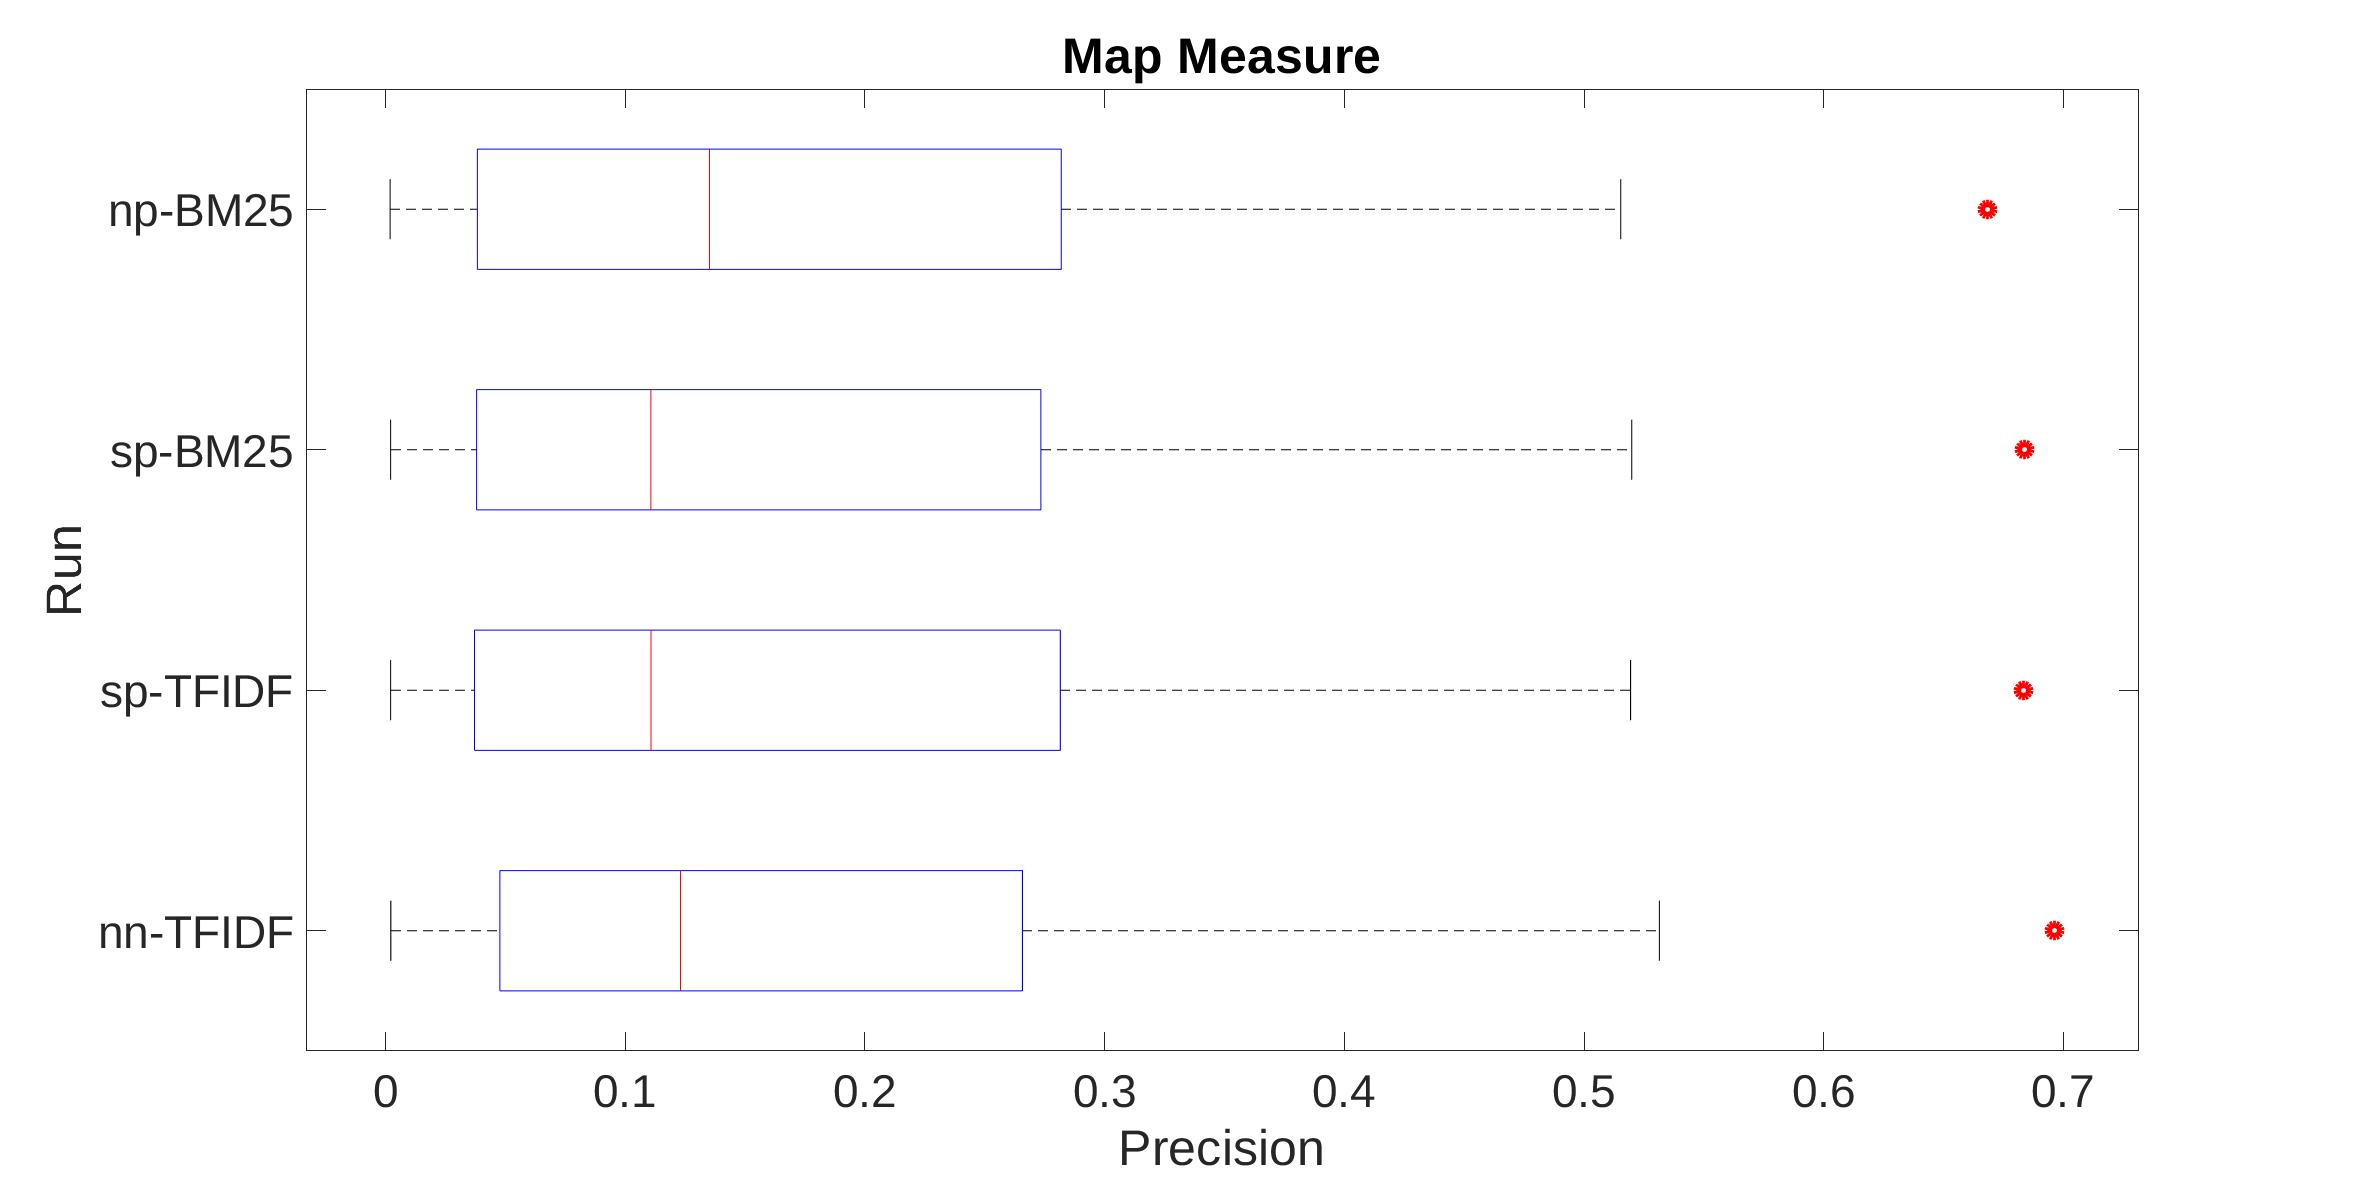
\includegraphics[width=\linewidth]{../Plots/mean-boxplot.jpeg}
\endminipage\hfill
\minipage{0.33\textwidth}
  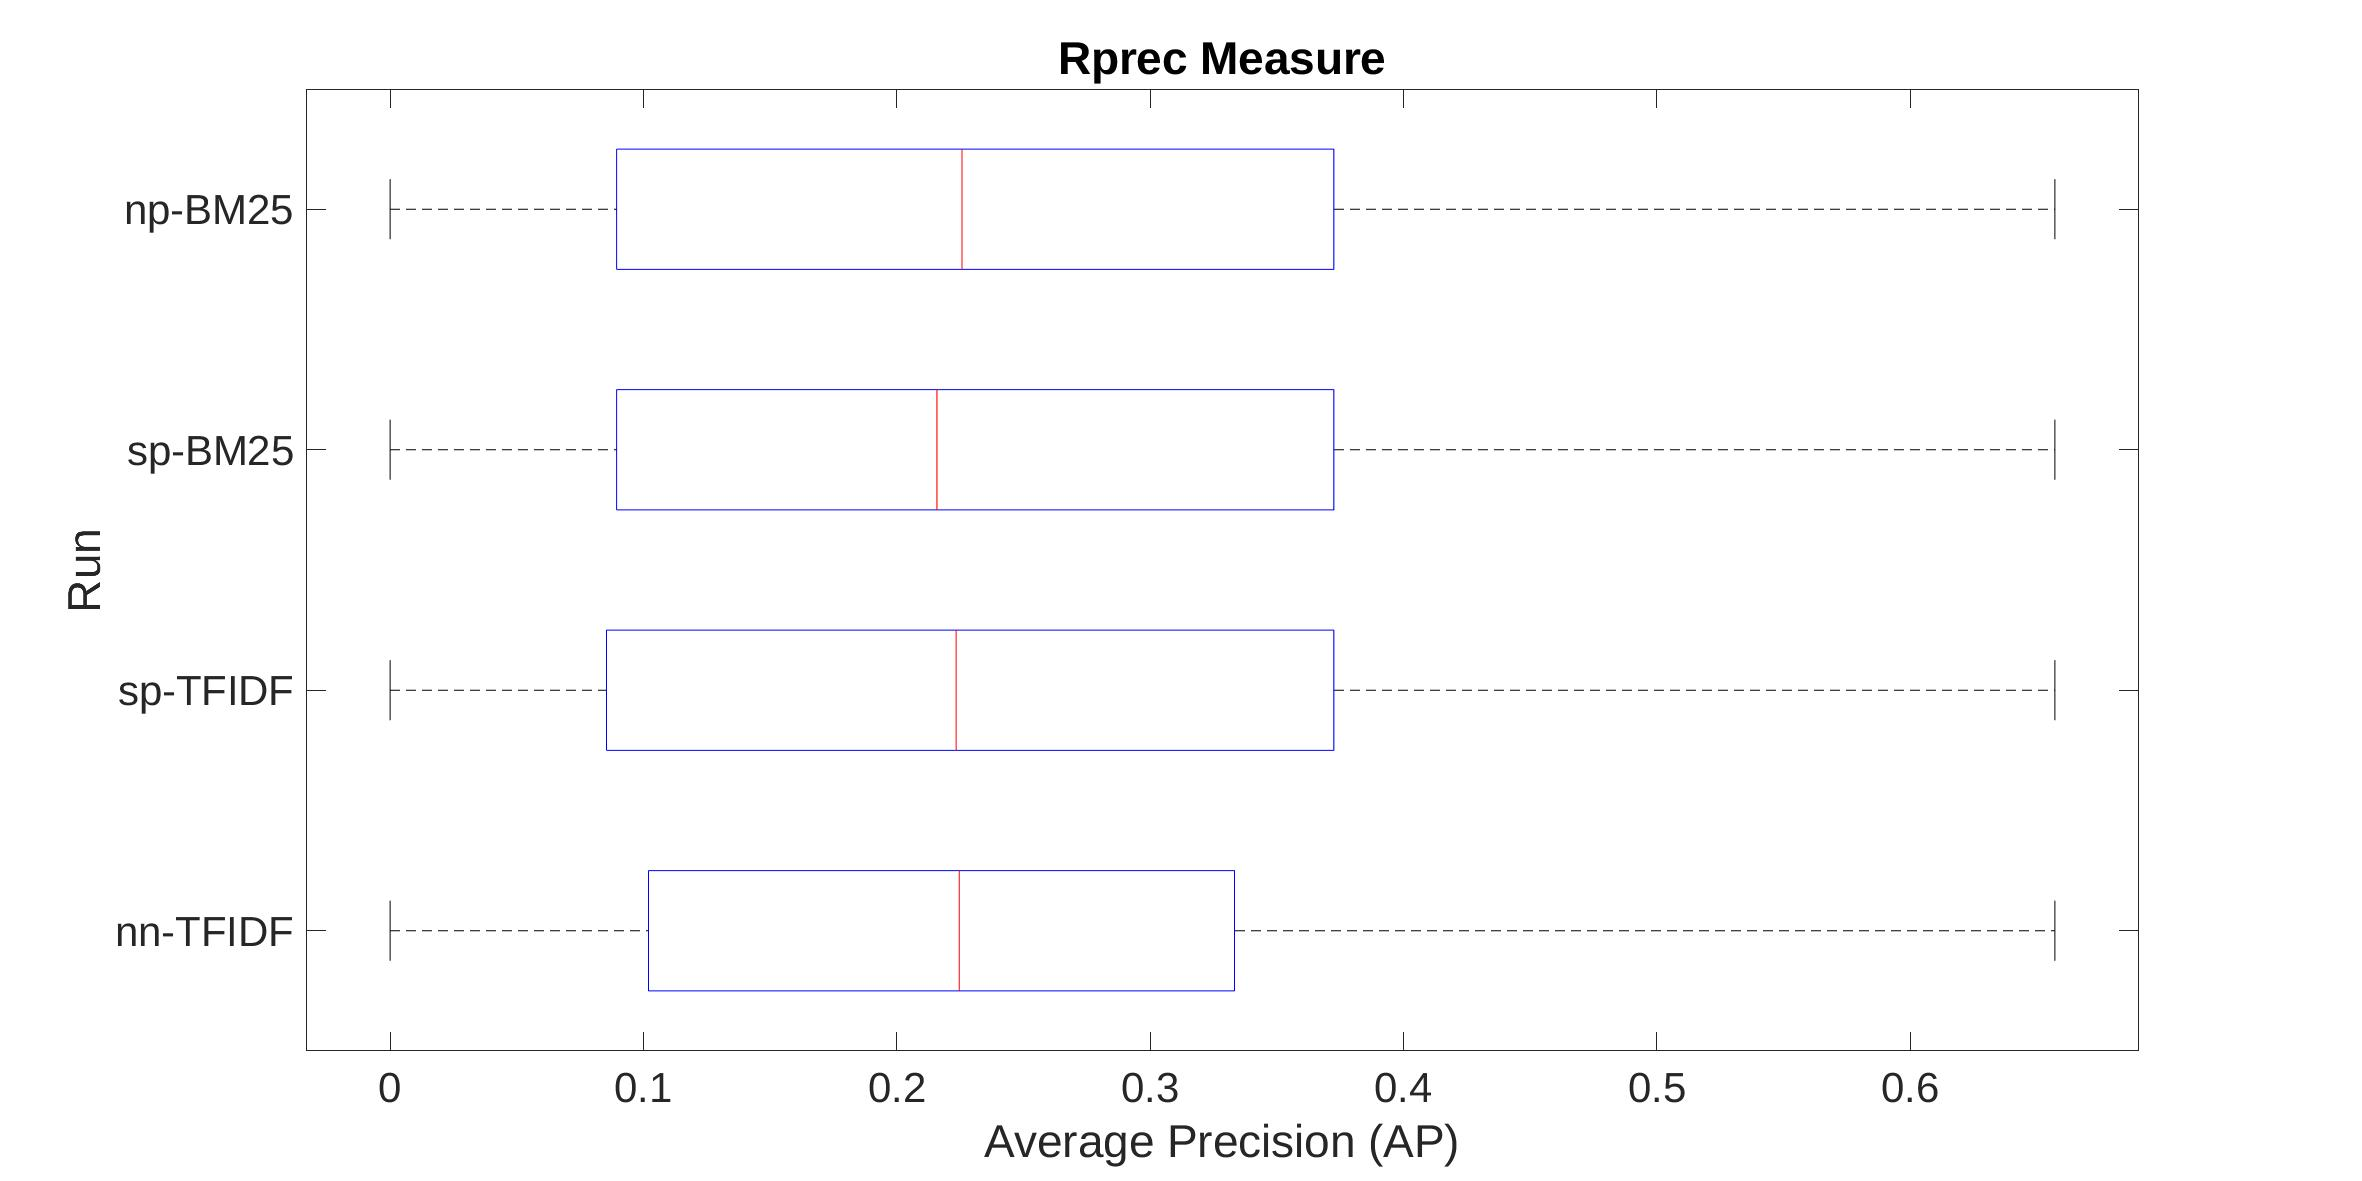
\includegraphics[width=\linewidth]{../Plots/rprec-boxplot.jpeg}
\endminipage\hfill
\minipage{0.33\textwidth}%
  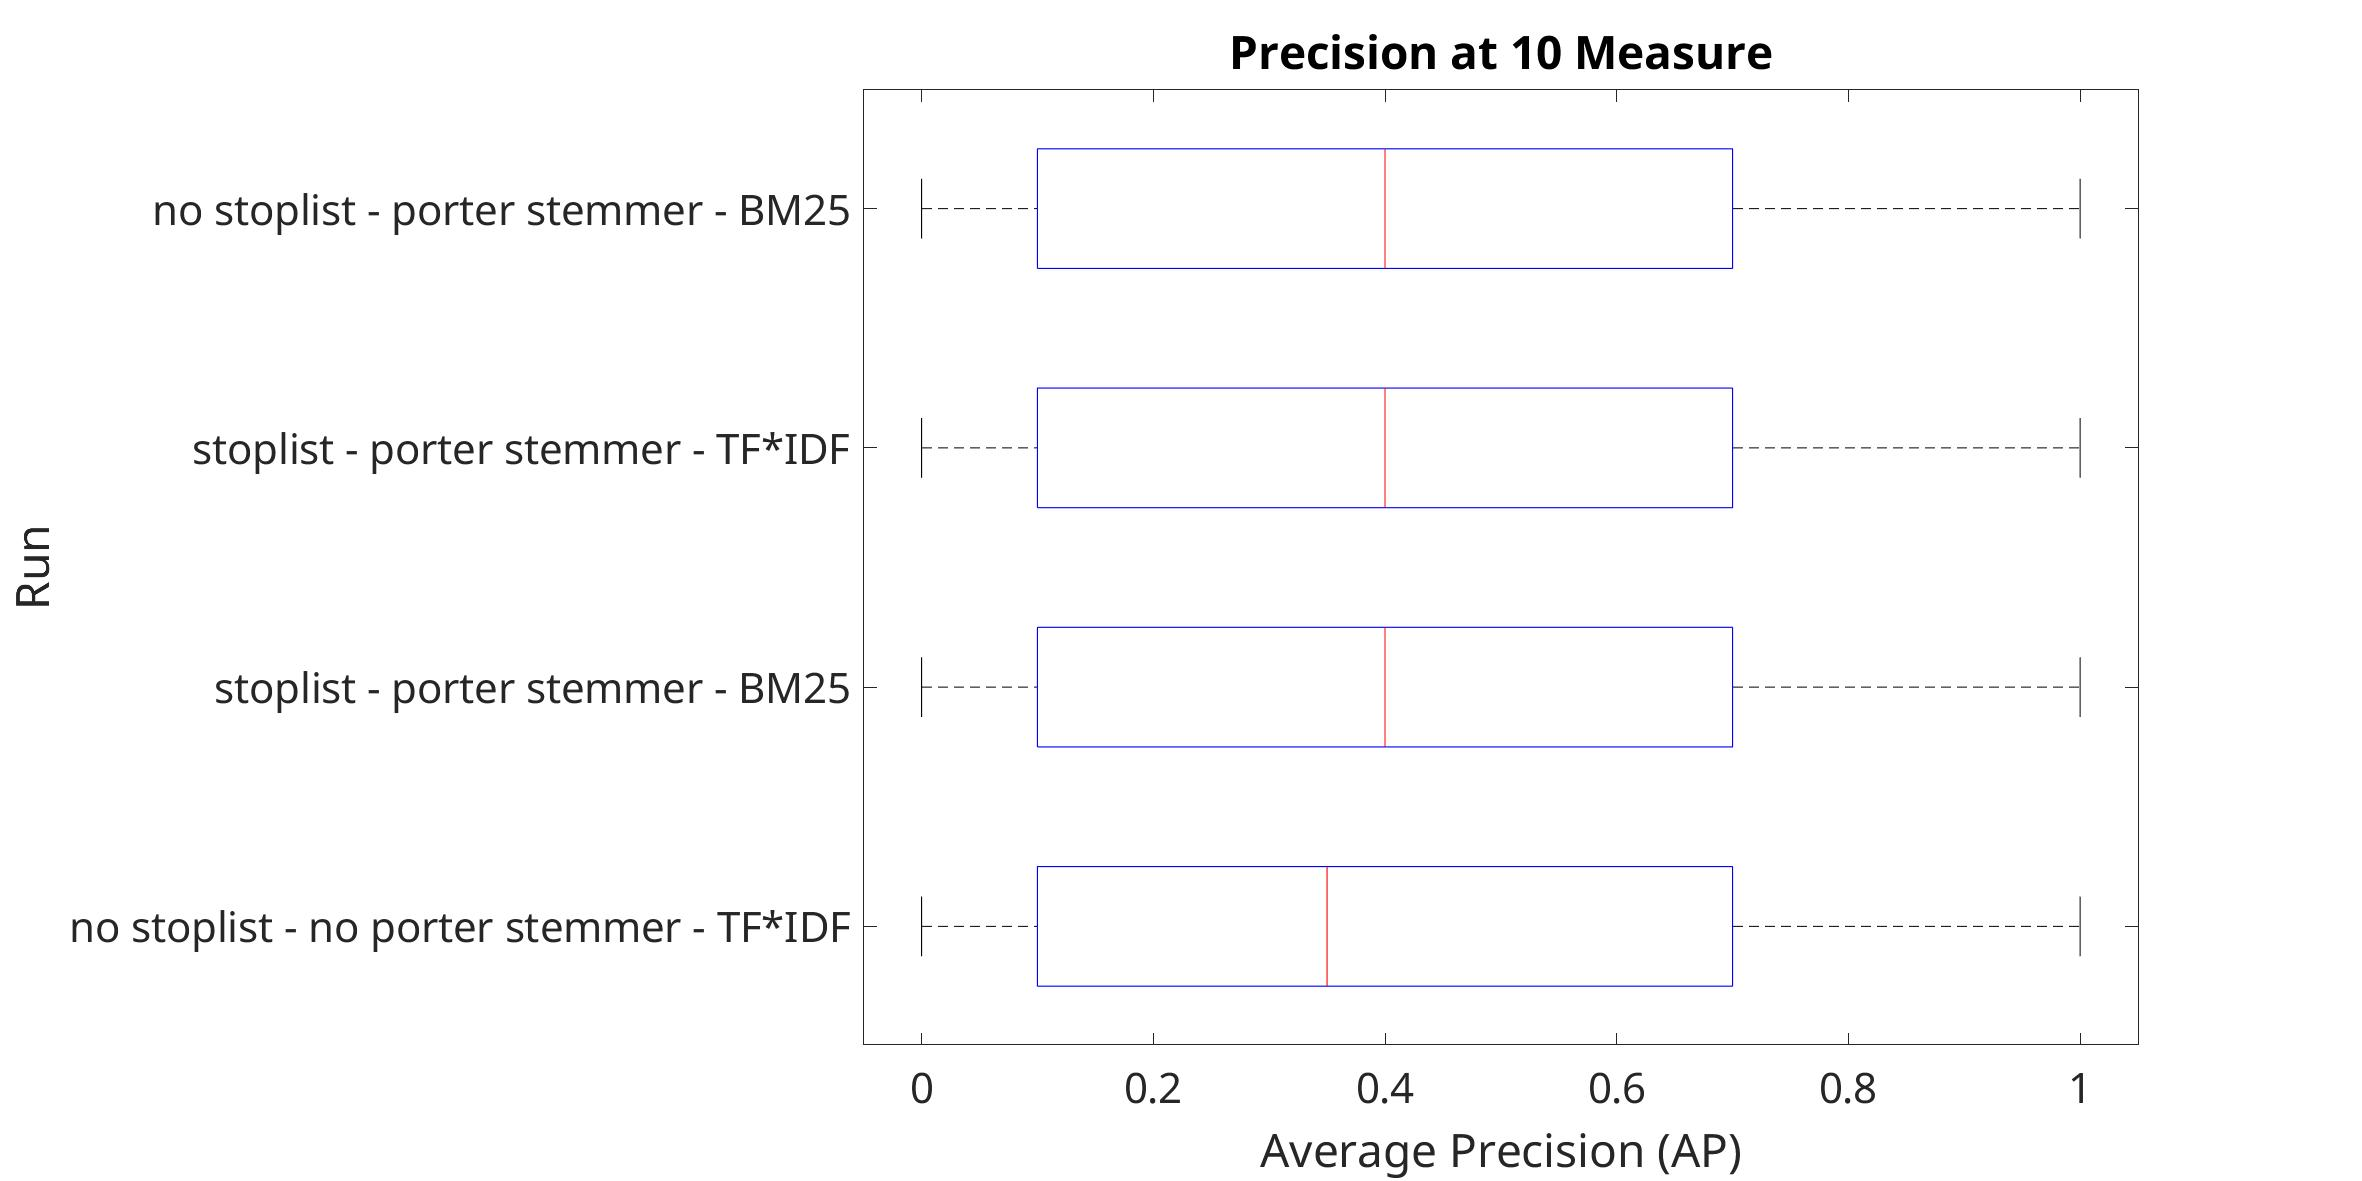
\includegraphics[width=\linewidth]{../Plots/p10-boxplot.jpeg}
\endminipage
\caption{Boxplot per le 3 diverse misure di precisione.}
\end{figure}
 
\begin{figure}[!htb]
\minipage{0.33\textwidth}
  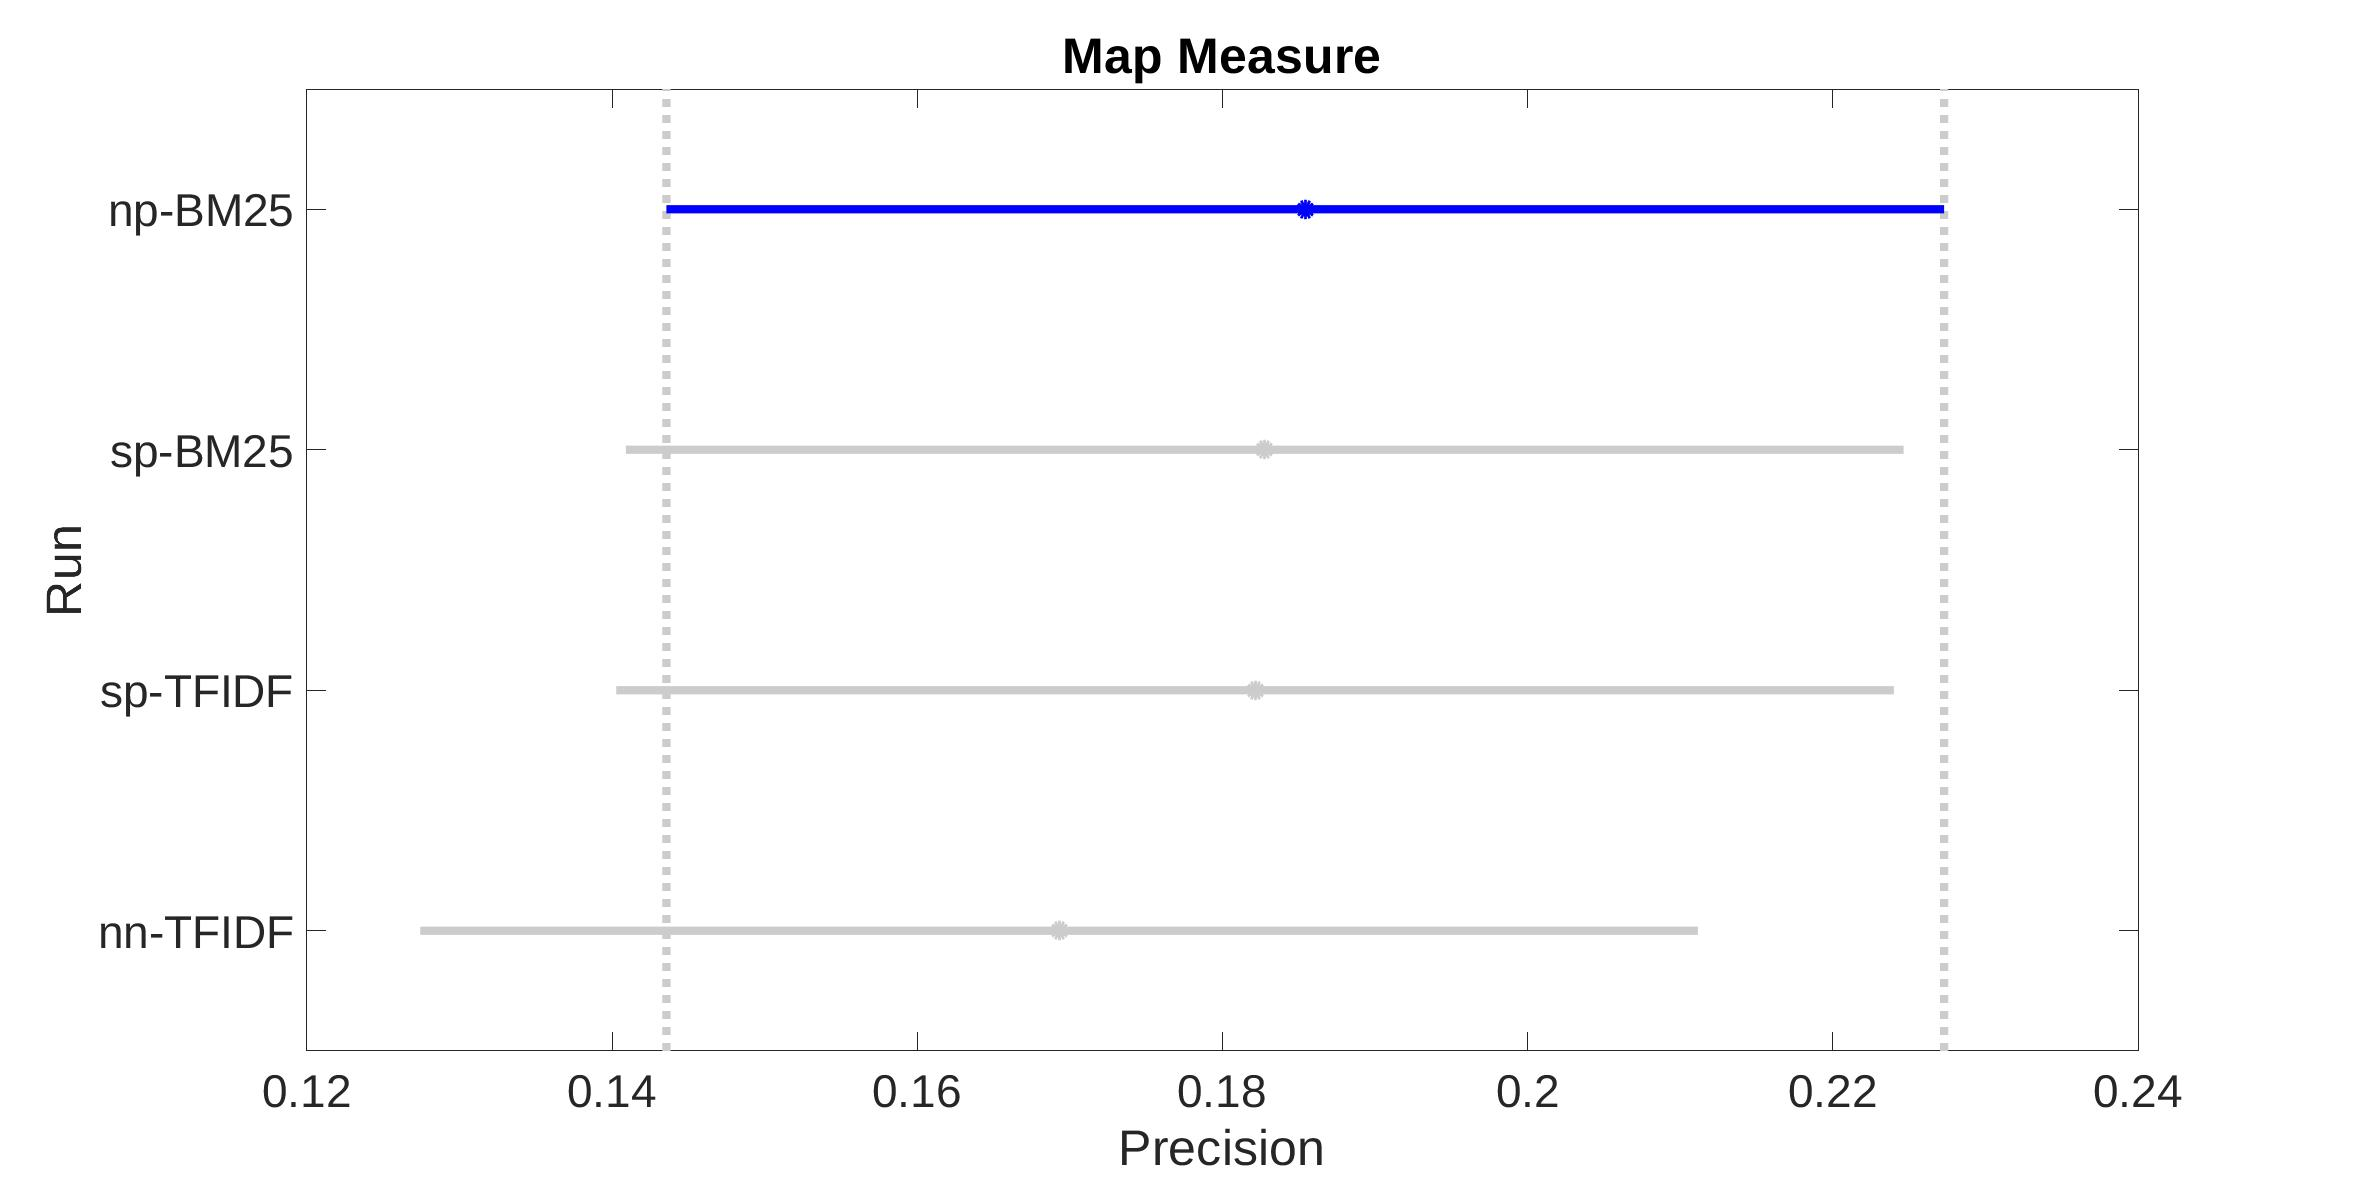
\includegraphics[width=\linewidth]{../Plots/mean-tukey.jpeg}
\endminipage\hfill
\minipage{0.33\textwidth}
  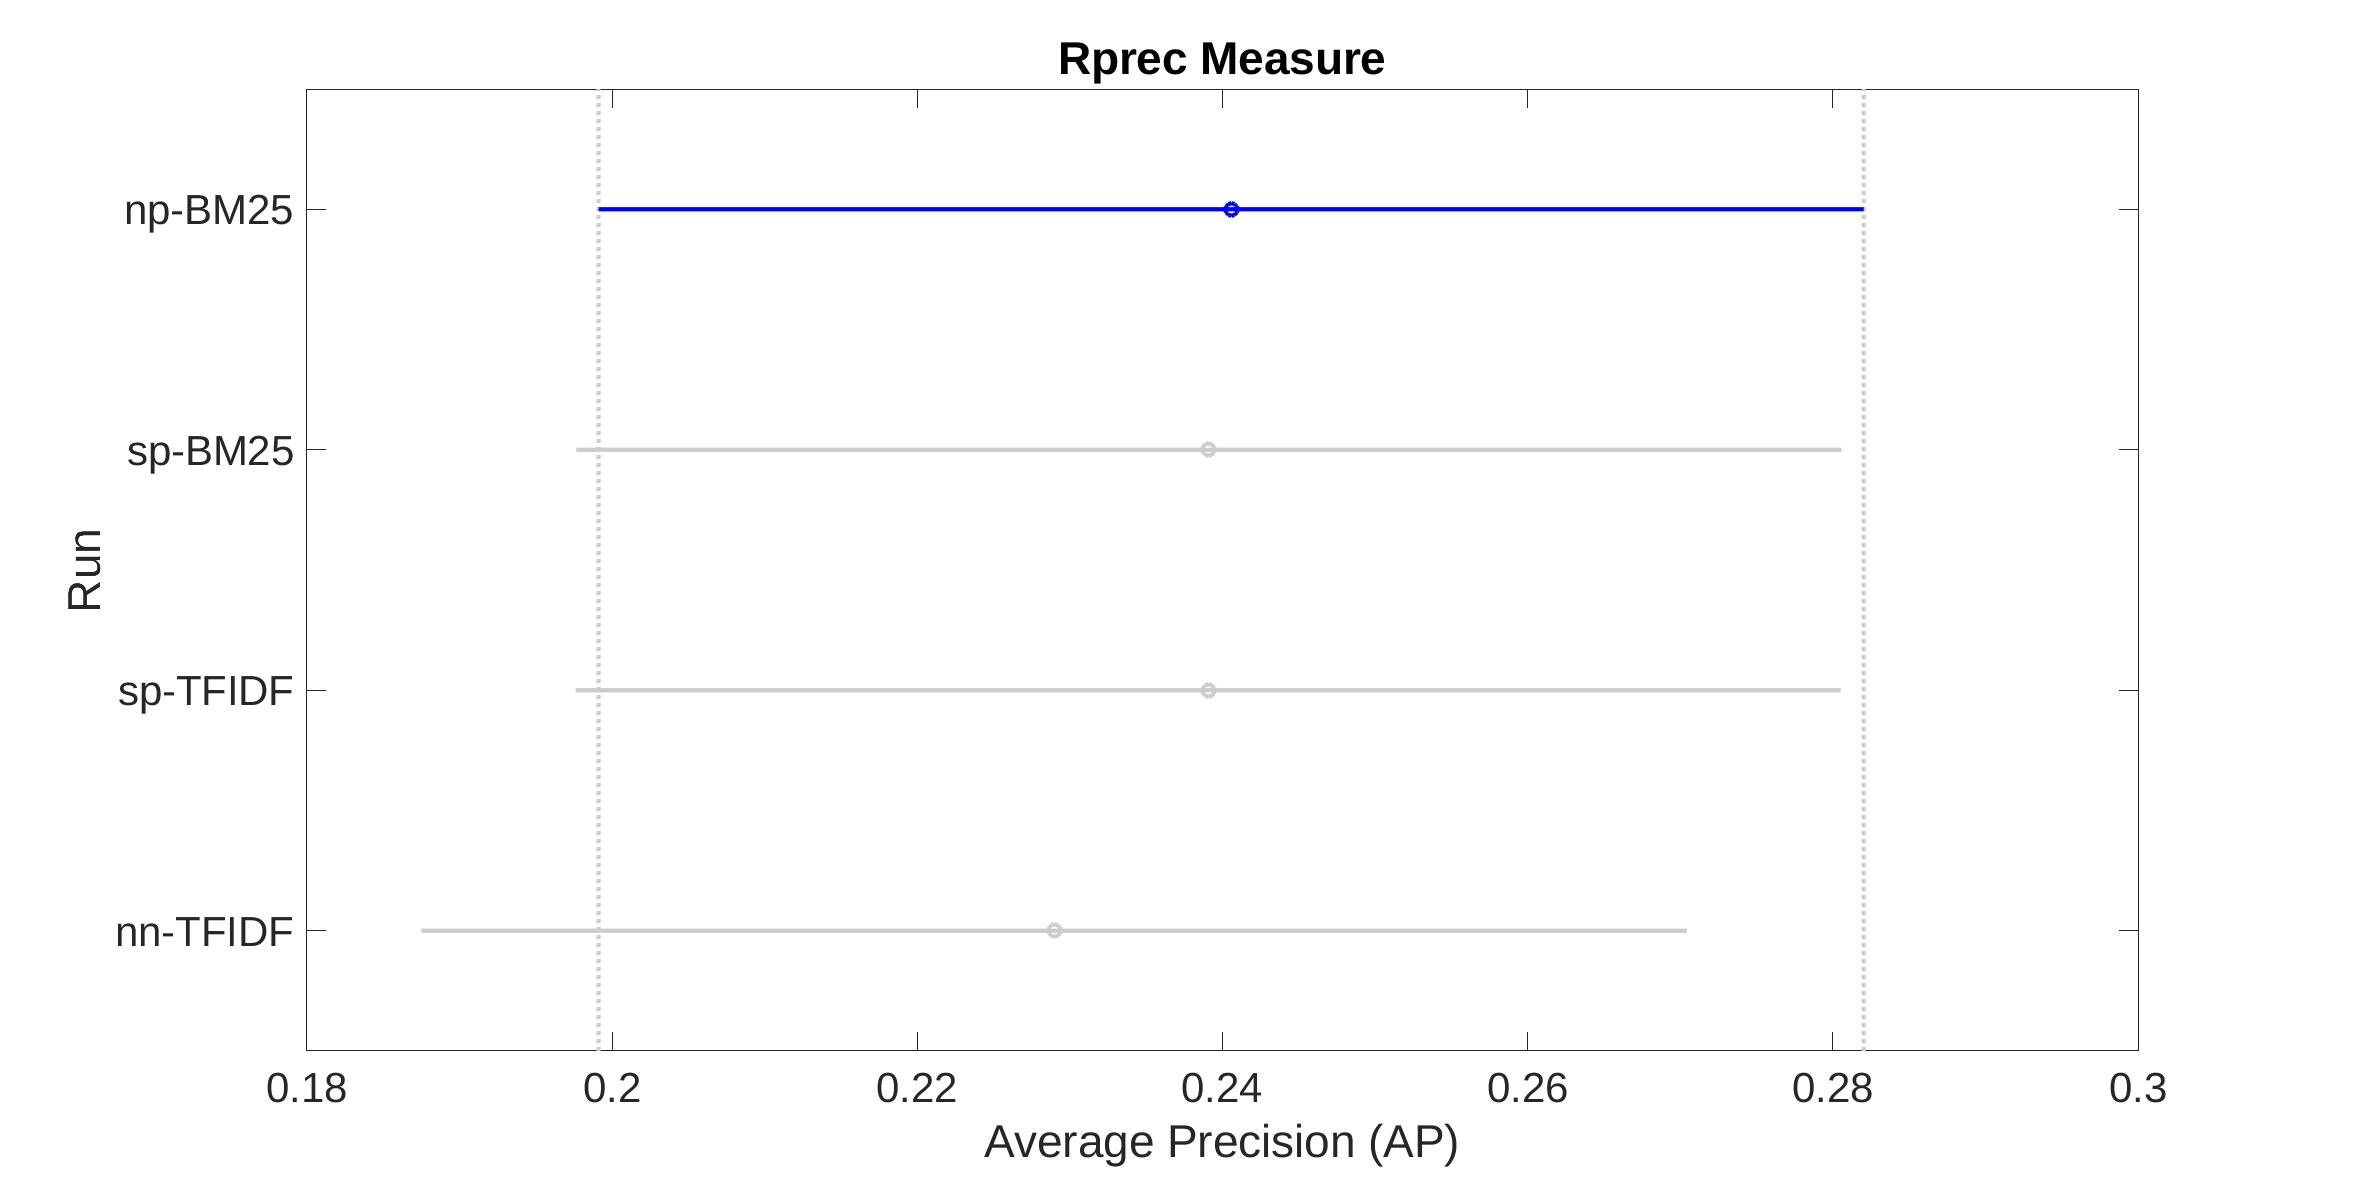
\includegraphics[width=\linewidth]{../Plots/rprec-tukey.jpeg}
\endminipage\hfill
\minipage{0.33\textwidth}%
  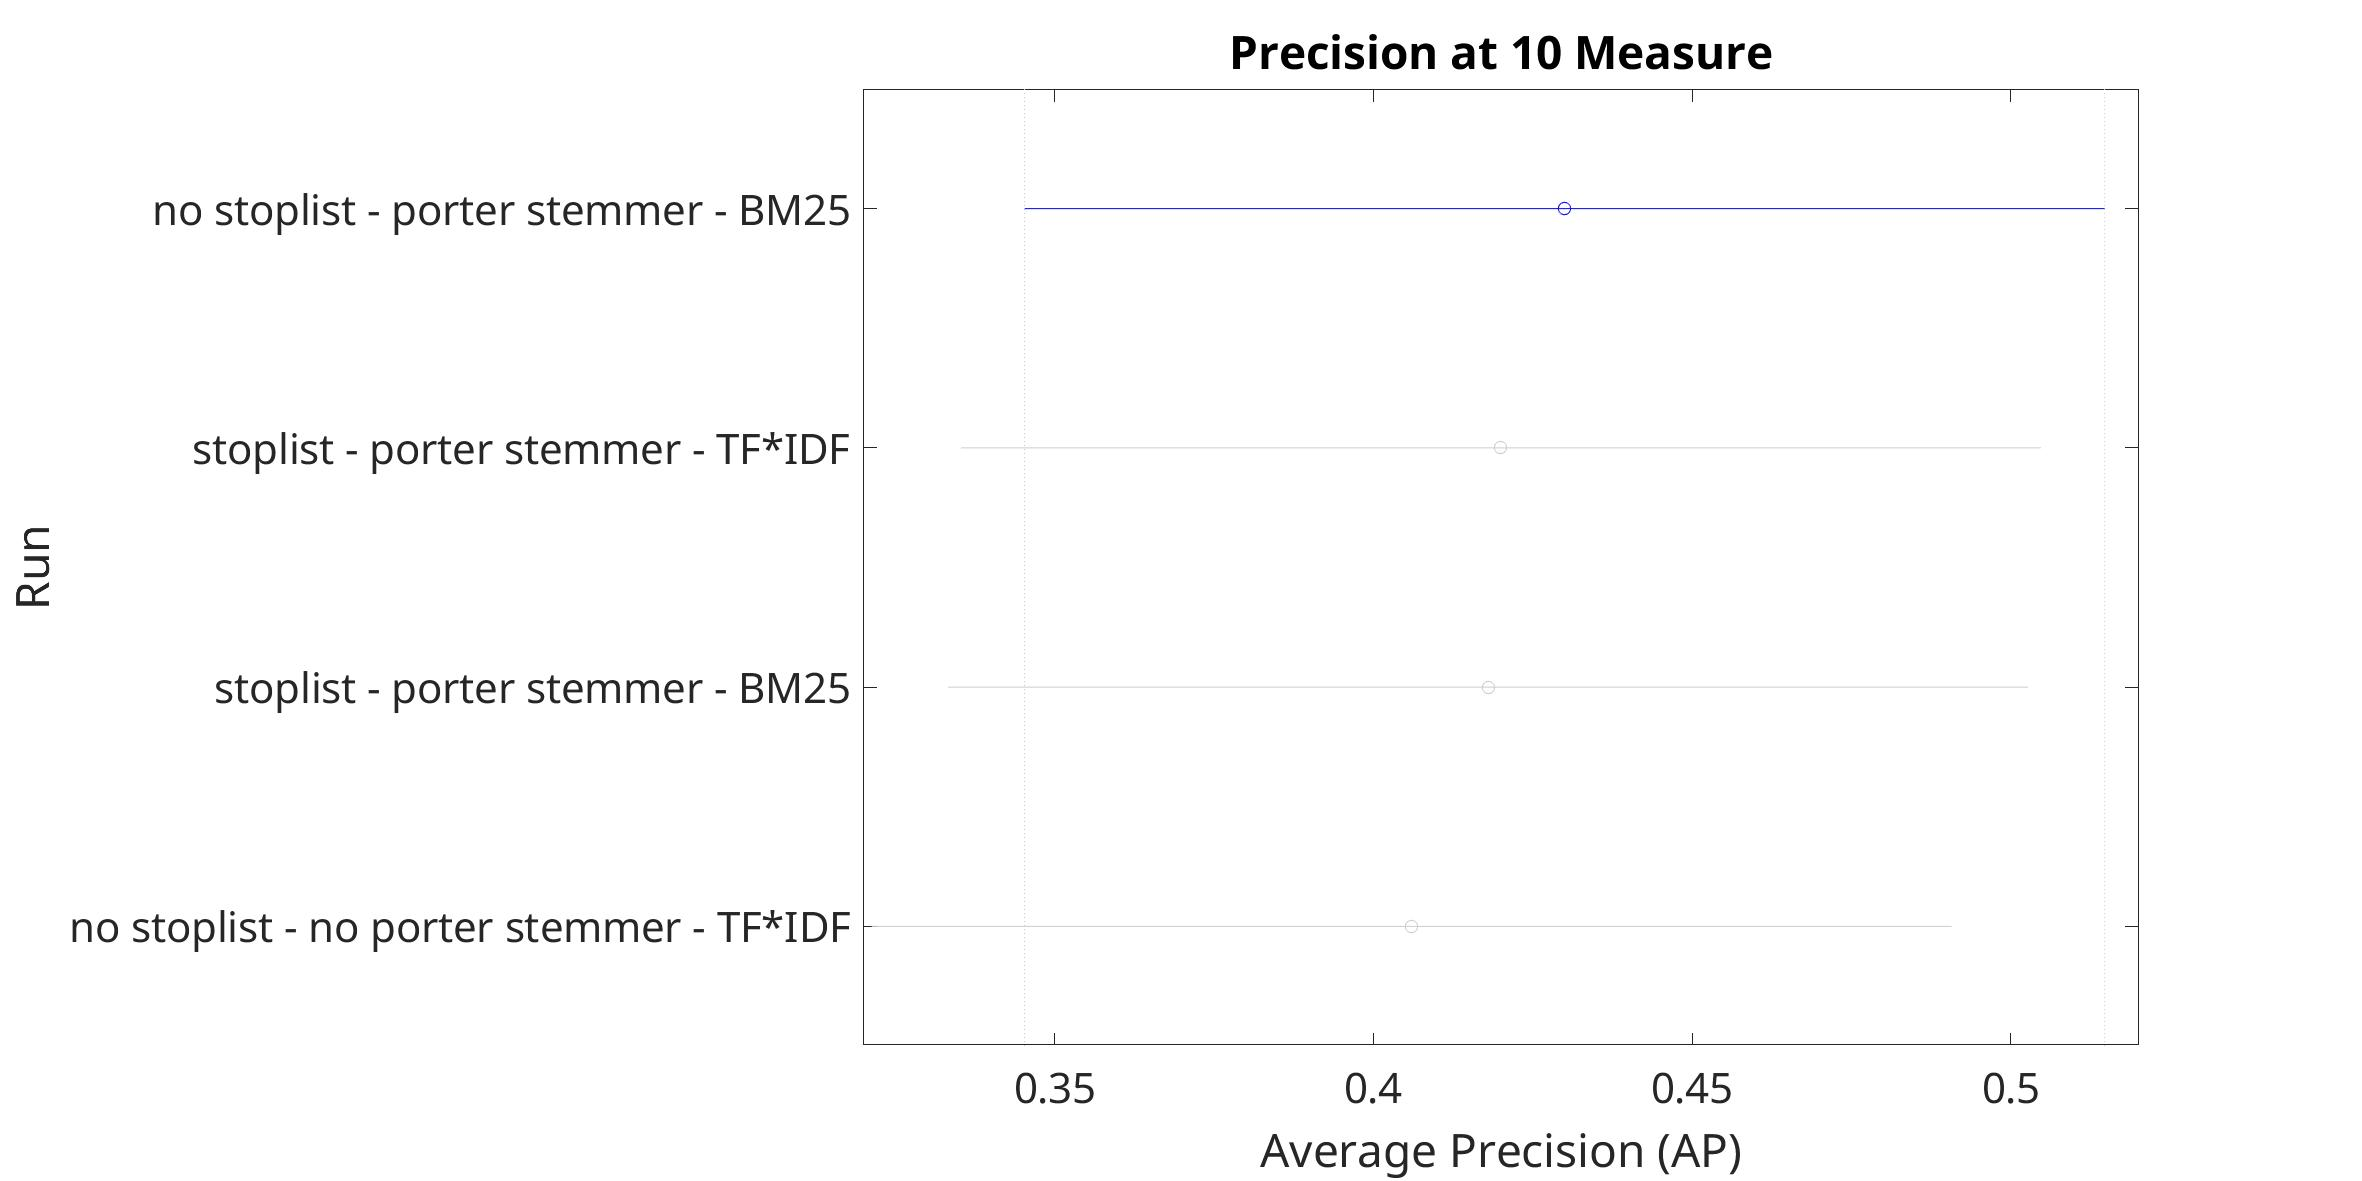
\includegraphics[width=\linewidth]{../Plots/p10-tukey.jpeg}
\endminipage
\caption{Tukey HSD test per le 3 diverse misure di precisione.}
\end{figure}

\noindent
I grafici riassumono quanto già parzialmente evidenziato nella sezione riguardante la valutazione, ovvero che np-BM25 ha una performance migliore rispetto agli altri casi analizzati. I boxplots sottolineano come np-BM25, sp-TFIDF e sp-BM25 abbiano una media molto simile, soprattutto nel caso della Precision at 10, dove i relativi valori della mediana e degli altri quartili sono identici, rispettivamente $q_{1/4}=0.1$ , $q_{2/4}=0.4$ e $q_{3/4}=0.7$. Il mantenimento delle stopwords e il mancato utilizzo del Porter stemmer, influenzato probabilmente anche dalla scelta di questa analisi di prendere in considerazione i termini con un basso indice di frequenza $idf$, ha invece diminuito la performance nel modello di pesatura TF*IDF, infatti in questo caso $q_{2/4}=0.35$.\\
Tale andamento si replica anche per la Mean Average Precision, nonostante gli outliers dovuti al topic 15, e la Recall Precision, dove nn-TFIDF ha un miglior primo e secondo quartile rispetto a sp-BM25 e sp-TFIDF, ma un terzo quartile nettamente inferiore.\\
Il test di Tukey conferma np-BM25 come la soluzione con la performance migliore rispetto alle altre 3, dovuto alla scelta di non tenere in considerazione il tag $DESC$ dei topic nel processo di valutazione e al non aver rimosso le stopwords dai documenti della collezione in fase di indicizzazione. Tukey evidenzia inoltre come np-BM25, sp-TFIDF e sp-BM25 abbiano una media molto simile, mentre nn-TFIDF è quello che si discosta più di tutti.\\
Altri interessanti plot sono disponibili all'interno della repository.

\end{document} 
